\begin{frame}
\frametitle{The WebGraph Framework}

 \begin{table}%[b]
\caption{Representación usando listado de sucesores directo y brechas.}
\centering
\tiny

\begin{tabular}{|l|l|l|l|}
	\toprule
	Nodo & Outd. & Sucesores & Usando brechas \\
	\midrule
	... & ... & ... & ... \\
	15 & 11 & 13, 15, 16, 17, 18, 19, 23, 24, 203, 315, 1034 & 3, 1, 0, 0, 0, 0, 3, 0, 178, 111, 718 \\
	16 & 10 & 15, 16, 17, 22, 23, 24, 315, 316, 317, 3041 & 1, 0, 0, 4, 0, 0, 290, 0, 0, 2723 \\
	17 & 0 &  &  \\
	18 & 5 & 13, 15, 16, 17, 50 & 9, 1, 0, 0, 32 \\
	... & ... & ... & ... \\
\end{tabular}
\end{table} 

\begin{table}%[t]
\caption{Representación usando copy list.}
\centering
\tiny

\begin{tabular}{|l|l|l|l|l|}
	\toprule
	Nodo & Outd. & Ref. & Copy list & Nodos extra \\
	\midrule
	... & ... & ... & ... & ... \\
	15 & 11 & 0 &  & 13, 15, 16, 17, 18, 19, 23, 24, 203, 315, 1034 \\
	16 & 10 & 1 & 01110011010 & 22, 316, 317, 3041 \\
	17 & 0 &  &  &  \\
	18 & 5 & 3 & 11110000000 & 50 \\
	... & ... & ... & ... & ... \\
\end{tabular}
\end{table} 

\end{frame}

\begin{frame}
\frametitle{The WebGraph Framework (2)}

\begin{table}%[t]
\caption{Representación usando copy blocks.}
\centering
\tiny

\begin{tabular}{|l|l|l|l|l|l|}
	\toprule
	Nodo & Outd. & Ref. & \# b & Copy blocks & Nodos extra \\
	\midrule
	... & ... & ... & ... & ... & ... \\
	15 & 11 & 0 &  &  & 13, 15, 16, 17, 18, 19, 23, 24, 203, 315, 1034 \\
	16 & 10 & 1 & 7 & 0, 0, 2, 1, 1, 0, 0 & 22, 316, 317, 3041 \\
	17 & 0 &  &  &  & \\
	18 & 5 & 3 & 1 & 4 & 50 \\
	... & ... & ... & ... & ... & ... \\
\end{tabular}
\end{table}

\begin{table}%[b]
\caption{Representación usando intervalos, con umbral $L_{min} = 2$.}
\centering
\tiny

\begin{tabular}{|l|l|l|l|l|l|l|l|l|}
	\toprule
	Nodo & Outd. & Ref. & \# b & Copy blocks & \# inter & Ext. izq. & Largo & Residuales \\
	\midrule
	... & ... & ... & ... & ... & ...  & ...  & ...  & ... \\
	15 & 11 & 0 &  &  & 2 & 0, 2 & 3, 0 & 5, 189, 111, 718 \\
	16 & 10 & 1 & 7 & 0, 0, 2, 1, 1, 0, 0 & 1 & 600 & 0 & 12, 3018 \\
	17 & 0 &  &  &  &  &  &  & \\
	18 & 5 & 3 & 1 & 4 & 0 &  &  & 50 \\
	... & ... & ... & ... & ... & ...  & ...  & ...  & ... \\
\end{tabular}
\end{table} 

\end{frame}


\begin{frame}
\frametitle{Graph Compression by BFS}

\begin{figure}%[b]
    	\centering
    	\begin{minipage}{0.45\textwidth}
    		\centering
    		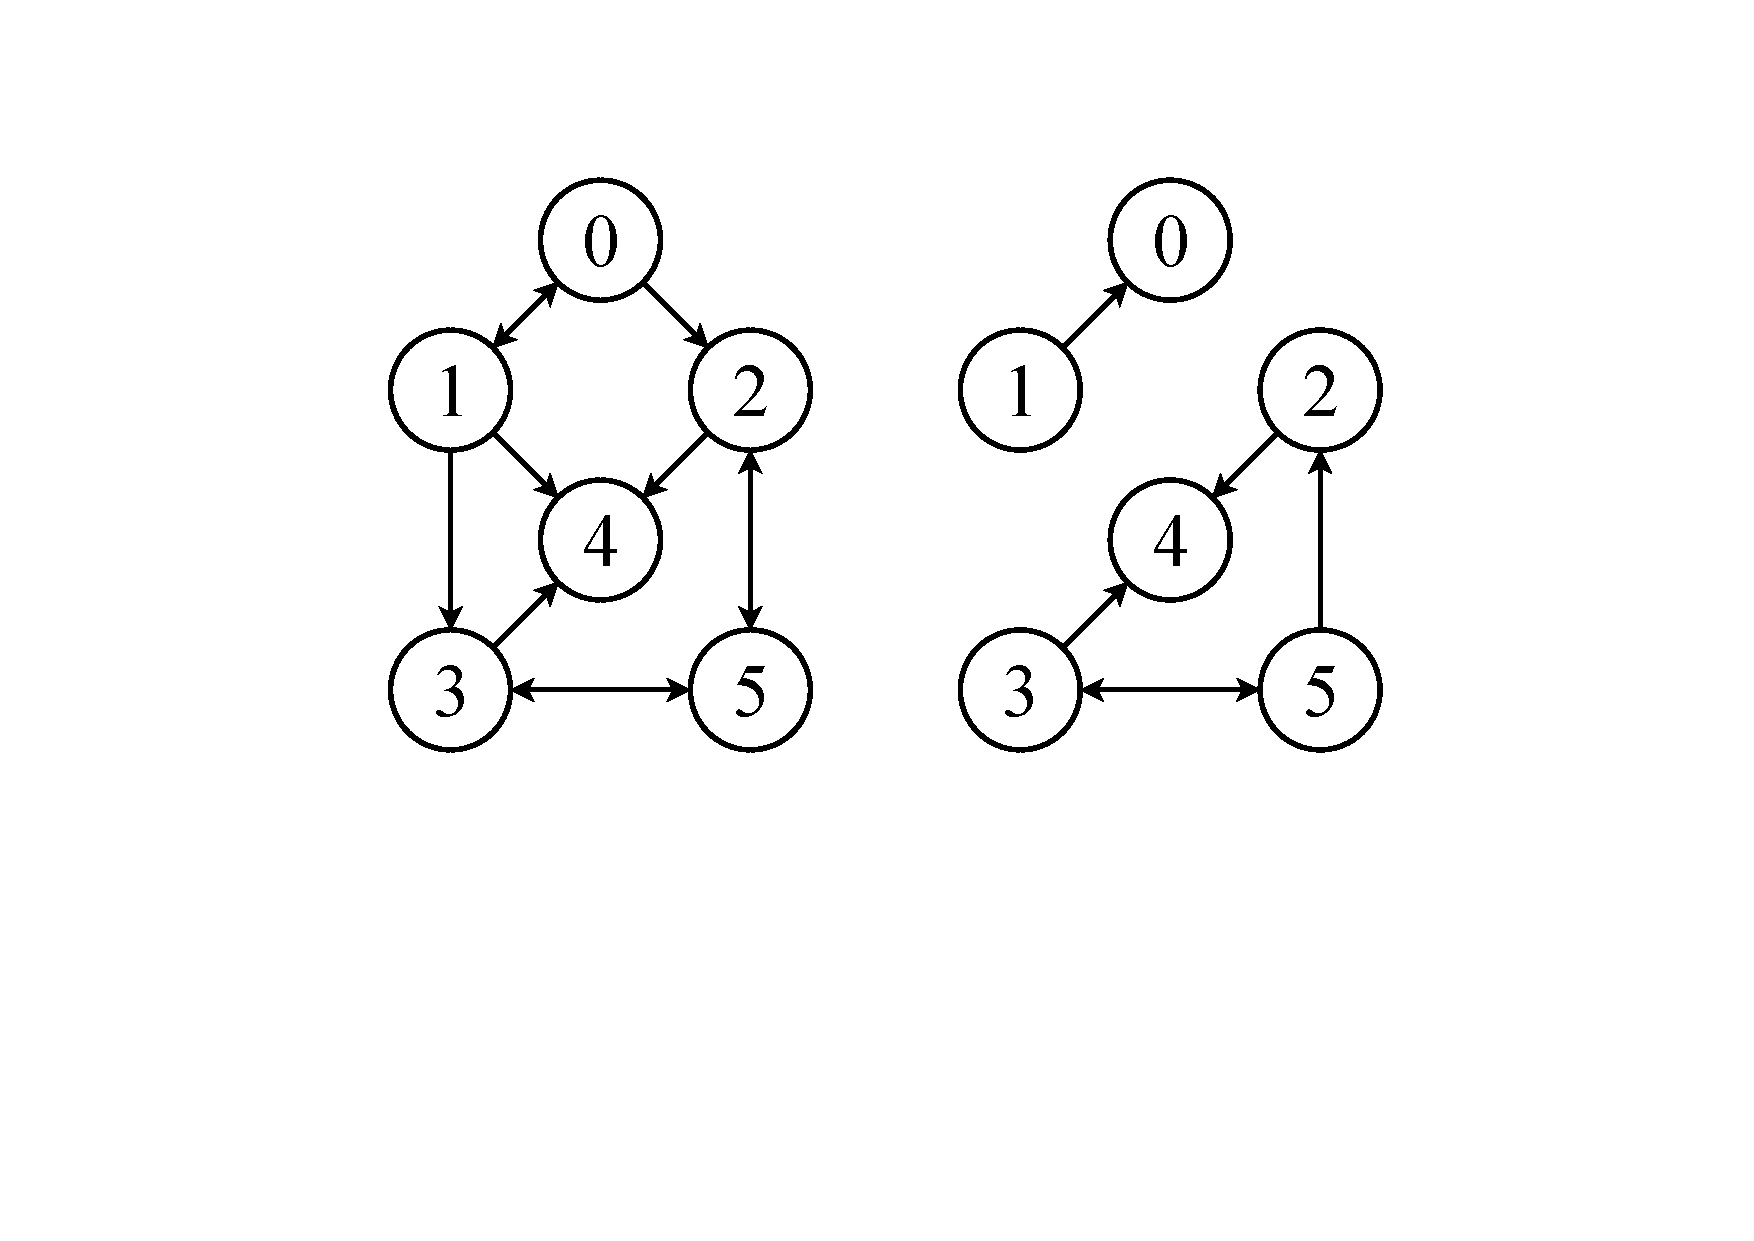
\includegraphics[scale=.3, clip, trim=180 230 440 80 ]{../img/arte/graphs-BFS-F1.pdf}
    		
    		(a)
    	\end{minipage}
    	\begin{minipage}{0.45\textwidth}
    		\centering
    		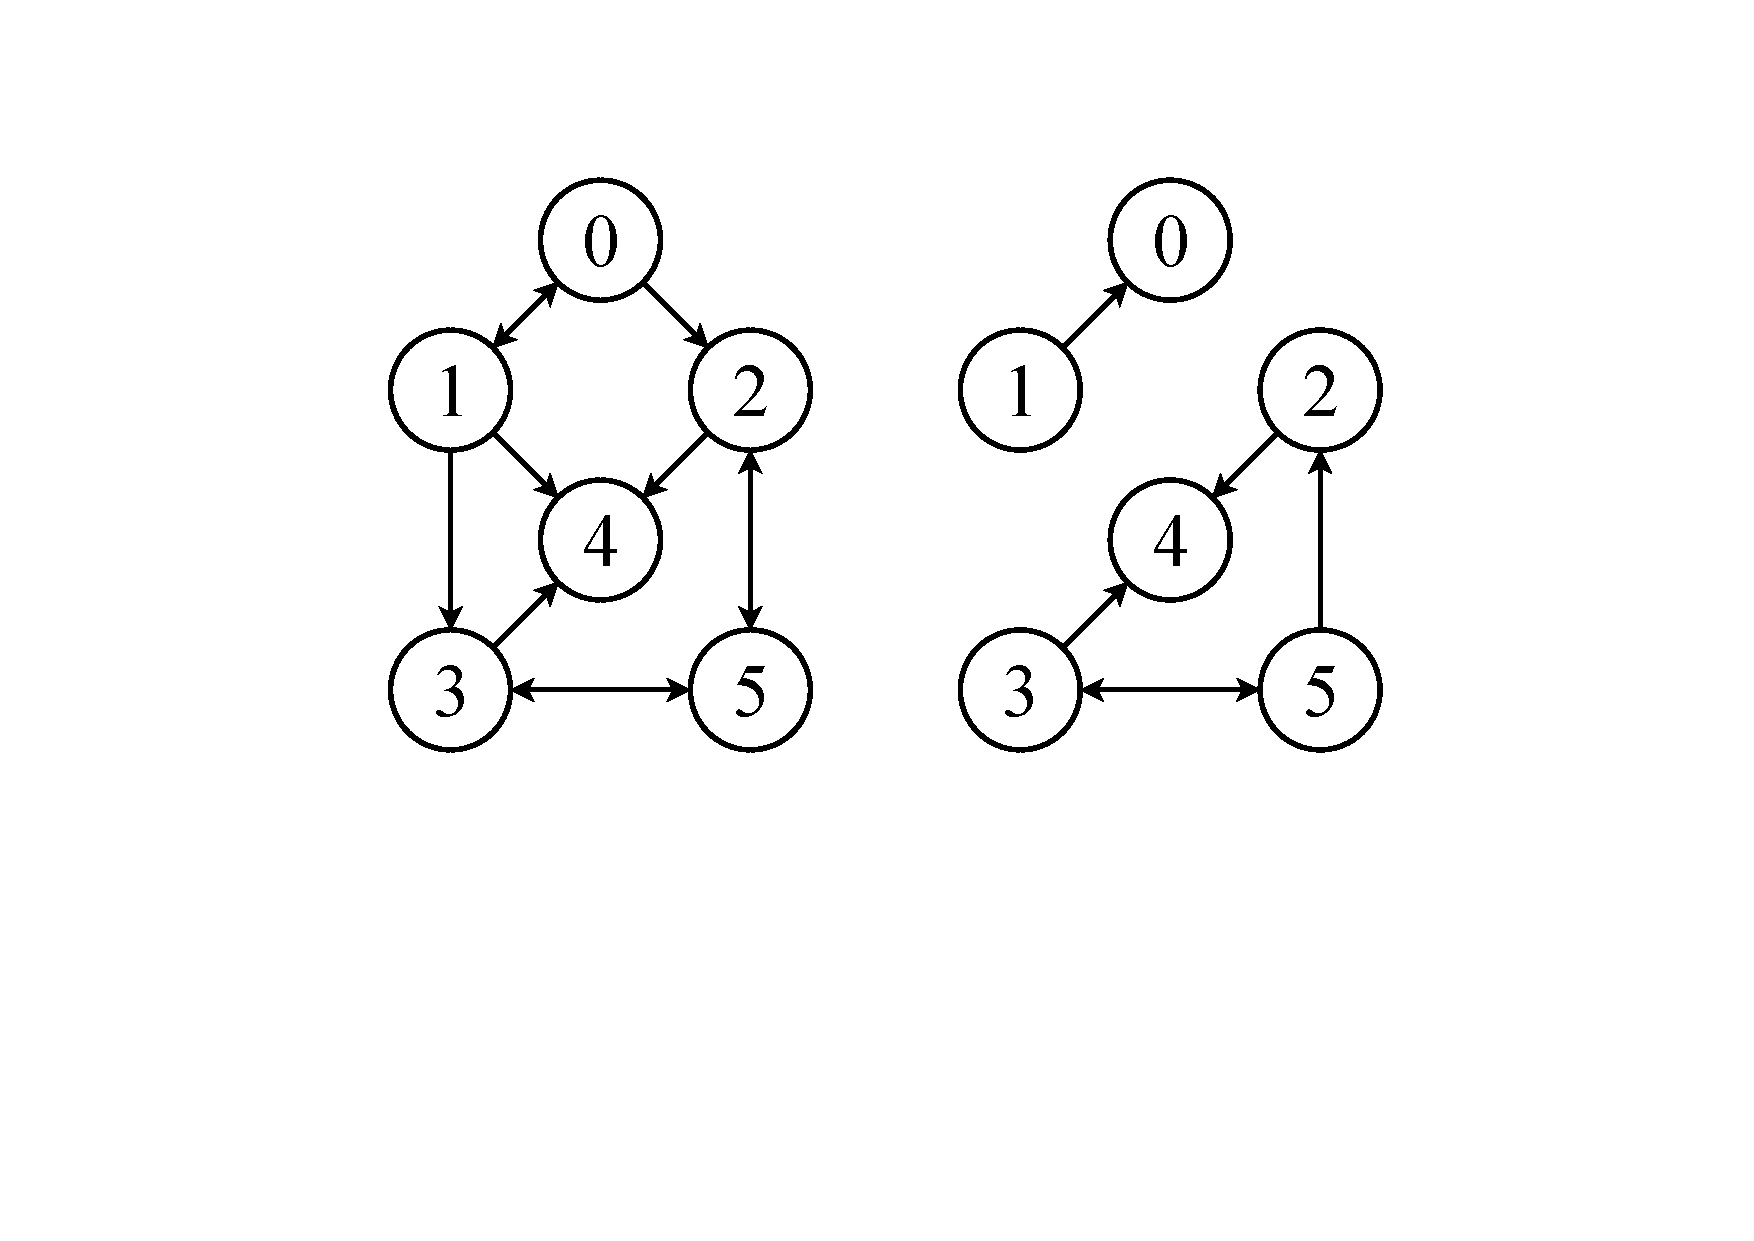
\includegraphics[scale=.3, clip, trim=450 230 170 80]{../img/arte/graphs-BFS-F1.pdf}
    		
    		$T = \{2, 2, 1, 0, 0, 0\}$
    		
    		(b)
    	\end{minipage}

    \caption{Ejemplo de Fase 1 de BFS. (a) Índices asignados a los nodos. (b) Aristas restantes después de BFS, junto listado de recorrido $T$.}
\end{figure}

\end{frame}

\begin{frame}
\frametitle{Graph Compression by BFS (2)}

 \begin{table}%[b]
\caption{Lista de adyacencia para BFS, $v_{i}$ el primer nodo de un trozo.}
\centering
\scriptsize

\begin{tabular}{|l|l|l|}
	\toprule
	Nodo & Grado & Adyacentes \\
	\midrule
	... & ... & ... \\
	i & 8 & 13, 15, 16, 17, 20, 21, 23, 24 \\
	i + 1 & 9 & 13, 15, 16, 17, 19, 20, 25, 31, 32 \\
	i + 2 & 0 &  \\
	i + 3 & 2 & 15, 16 \\
	... & ... & ... \\
\end{tabular}
\end{table} 

\begin{table}%[b]
\caption{Codificación BFS del listado de adyacencia.}
\centering
\scriptsize

\begin{tabular}{|l|l|l|}
	\toprule
	Nodo & Grado & Adyacentes \\
	\midrule
	... & ... & ... \\
	i & 8 & $\phi13$, $\phi1$, $\phi0$, $\phi0$, $\phi2$, $\phi0$, $\phi1$, $\phi0$ \\
	i + 1 & 9 & $\beta0$, $\beta0$, $\beta0$, $\beta0$, $\chi0$, $\alpha0$, $\beta2$, $\phi5$, $\phi0$ \\
	i + 2 & 0 &  \\
	i + 3 & 2 & $\beta2$, $\alpha0$ \\
	... & ... & ... \\
\end{tabular}
\end{table} 

\end{frame}

\begin{frame}
\frametitle{Graph Compression by BFS (3)}

 \begin{table}%[b]
\caption{Ejemplo de redundancias a explotar en listado de adyacencia de BFS.}
\centering
\tiny

\begin{tabular}{|l|llllllllll|}
	\toprule
	Grado & \multicolumn{9}{l}{Adyacentes} & \\
	\midrule
	\cellcolor{blanco} ... & \multicolumn{9}{l}{\cellcolor{blanco} ...} & \\
	\cellcolor{blanco} 0 & \multicolumn{9}{l}{} & \\
	\cellcolor{rojo} 9 & \cellcolor{blanco} $\beta1,$ & \cellcolor{cafe} $\phi1,$ & \cellcolor{cafe} $\phi1,$ & \cellcolor{cafe} $\phi1,$ & \cellcolor{blanco} $\phi0,$ & \cellcolor{blanco} $\phi1,$ & \cellcolor{blanco} $\phi1,$ & \cellcolor{blanco} $\phi1,$ & \cellcolor{blanco} $\phi1,$ & \\
    \cellcolor{rojo} 9 & \cellcolor{azul} $\beta0,$ & \cellcolor{azul} $\beta1,$ & \cellcolor{azul} $\beta0,$ & \cellcolor{azul} $\beta0,$ & \cellcolor{azul} $\beta0,$ & \cellcolor{azul} $\beta0,$ & \cellcolor{azul} $\beta0,$ & \cellcolor{azul} $\beta0,$ & \cellcolor{blanco} $\beta2,$ & \\
    \cellcolor{blanco} 10 &  \cellcolor{azul} $\beta0,$ & \cellcolor{azul} $\beta1,$ & \cellcolor{azul} $\beta0,$ & \cellcolor{azul} $\beta0,$ & \cellcolor{azul} $\beta0,$ & \cellcolor{azul} $\beta0,$ & \cellcolor{azul} $\beta0,$ & \cellcolor{azul} $\beta0,$  & \cellcolor{blanco} $\beta1,$ & \cellcolor{blanco} $\phi903$ \\
    \cellcolor{blanco} 10 &  \cellcolor{azul} $\beta0,$ & \cellcolor{azul} $\beta1,$ & \cellcolor{azul} $\beta0,$ & \cellcolor{azul} $\beta0,$ & \cellcolor{azul} $\beta0,$ & \cellcolor{azul} $\beta0,$ & \cellcolor{azul} $\beta0,$ & \cellcolor{azul} $\beta0,$  & \cellcolor{blanco} $\beta223,$ & \cellcolor{blanco} $\phi900$ \\
    \cellcolor{blanco} 10 &  \cellcolor{azul} $\beta0,$ & \cellcolor{azul} $\beta1,$ & \cellcolor{azul} $\beta0,$ & \cellcolor{azul} $\beta0,$ & \cellcolor{azul} $\beta0,$ & \cellcolor{azul} $\beta0,$ & \cellcolor{azul} $\beta0,$ & \cellcolor{azul} $\beta0,$  & \cellcolor{blanco} $\beta1,$ & \cellcolor{blanco} $\alpha0$ \\
    \cellcolor{amarillo} 10 & \cellcolor{verde} $\beta0,$ & \cellcolor{verde} $\beta1,$ & \cellcolor{verde} $\beta0,$ & \cellcolor{verde} $\beta0,$ & \cellcolor{verde} $\beta0,$ & \cellcolor{verde} $\beta0,$ & \cellcolor{verde} $\beta0,$ & \cellcolor{verde} $\beta0,$ & \cellcolor{amarillo} $\beta1,$ & \cellcolor{amarillo} $\beta0$ \\
    \cellcolor{amarillo} 10 & \cellcolor{verde} $\beta0,$ & \cellcolor{verde} $\beta1,$ & \cellcolor{verde} $\beta0,$ & \cellcolor{verde} $\beta0,$ & \cellcolor{verde} $\beta0,$ & \cellcolor{verde} $\beta0,$ & \cellcolor{verde} $\beta0,$ & \cellcolor{verde} $\beta0,$ & \cellcolor{amarillo} $\beta1,$ & \cellcolor{amarillo} $\beta0$ \\
    \cellcolor{amarillo} 10 & \cellcolor{verde} $\beta0,$ & \cellcolor{verde} $\beta1,$ & \cellcolor{verde} $\beta0,$ & \cellcolor{verde} $\beta0,$ & \cellcolor{verde} $\beta0,$ & \cellcolor{verde} $\beta0,$ & \cellcolor{verde} $\beta0,$ & \cellcolor{verde} $\beta0,$ & \cellcolor{amarillo} $\beta1,$ & \cellcolor{amarillo} $\beta0$ \\
    \cellcolor{amarillo} 10 & \cellcolor{verde} $\beta0,$ & \cellcolor{verde} $\beta1,$ & \cellcolor{verde} $\beta0,$ & \cellcolor{verde} $\beta0,$ & \cellcolor{verde} $\beta0,$ & \cellcolor{verde} $\beta0,$ & \cellcolor{verde} $\beta0,$ & \cellcolor{verde} $\beta0,$ & \cellcolor{amarillo} $\beta1,$ & \cellcolor{amarillo} $\beta0$ \\
    \cellcolor{blanco} 10 &  \cellcolor{azul} $\beta0,$ & \cellcolor{azul} $\beta1,$ & \cellcolor{azul} $\beta0,$ & \cellcolor{azul} $\beta0,$ & \cellcolor{azul} $\beta0,$ & \cellcolor{azul} $\beta0,$ & \cellcolor{azul} $\beta0,$ & \cellcolor{azul} $\beta0,$  & \cellcolor{blanco} $\alpha76,$ & \cellcolor{blanco} $\alpha232$ \\
    \cellcolor{blanco} 9 &  \cellcolor{azul} $\beta0,$ & \cellcolor{azul} $\beta1,$ & \cellcolor{azul} $\beta0,$ & \cellcolor{azul} $\beta0,$ & \cellcolor{azul} $\beta0,$ & \cellcolor{azul} $\beta0,$ & \cellcolor{azul} $\beta0,$ & \cellcolor{azul} $\beta0,$  & \cellcolor{blanco} $\beta0$ & \\
	\cellcolor{blanco} ... & \multicolumn{9}{l}{\cellcolor{blanco} ...} & \\
\end{tabular}
\end{table} 

\end{frame}

\begin{frame}
\frametitle{Graph Compression by BFS (4)}

 \begin{table}%[b]
\caption{Ejemplo de redundancias codificadas de BFS.}
\centering
\scriptsize

\begin{tabular}{|l|l|llll|}
	\toprule
	Líneas & Grado & \multicolumn{3}{l}{Enlaces} &  \\
	\midrule
	... & ... & ... & & &  \\
	0 & 0 & & & & \\
	0 & 9 & $\beta7$, & $\phi\:\Sigma\:2\:1\:1$, & $\phi0$, & $\phi\:\Sigma\:2\:1\:2$ \\
	0 & 0 & $\beta\:\Sigma\:3\:0\:7\:5$, & $\beta1$, & $\beta\:\Sigma\:2\:0\:4$, & $\beta2$ \\
	0 & 1 & $\beta1$, & $\phi903$ & & \\
	0 & 0 & $\beta223$, & $\phi900$ & & \\
	0 & 0 & $\beta1$, & $\alpha0$ & & \\
	3 & 0 & $\beta1$, & $\beta0$ & & \\
	0 & 0 & $\alpha76$, & $\alpha232$ & & \\
	0 & -1 & $\beta0$ & & & \\
	... & ... & ... & & &  \\
\end{tabular}
\end{table} 

\end{frame}


\begin{frame}
\frametitle{Using Re-Pair}

 \begin{table}%[b]
\caption{Ejemplo de Re-Pair. Las reglas en la tabla conforman el diccionario asociado a la compresión.}
\label{table:repair}
\centering
\footnotesize

\begin{tabular}{|l|l|}
	\toprule
	Reglas & String \\
	\midrule
	 & $singing.do.wah.diddy.diddy.dum.diddy.do$ \\
	$A \rightarrow .d$ & $singingAo.wahAiddyAiddyAumAiddyAo$ \\
	$B \rightarrow dd$ & $singingAo.wahAiByAiByAumAiByAo$ \\
	$C \rightarrow Ai$ & $singingAo.wahCByCByAumCByAo$ \\
	$D \rightarrow By$ & $singingAo.wahCDCDAumCDAo$ \\
	$E \rightarrow CD$ & $singingAo.wahEEAumEAo$ \\
	$F \rightarrow in$ & $sFgFgAo.wahEEAumEAo$ \\
	$G \rightarrow Ao$ & $sFgFgG.wahEEAumEG$ \\
	$H \rightarrow Fg$ & $sHHG.wahEEAumEG$ \\
	\bottomrule
\end{tabular}
\end{table} 

\end{frame}

\begin{frame}
\frametitle{Using Re-Pair (2)}

\begin{figure}%[b]
    	\centering
    	\begin{minipage}{1\textwidth}
    		\begin{minipage}{.6\textwidth}
    			\centering
    			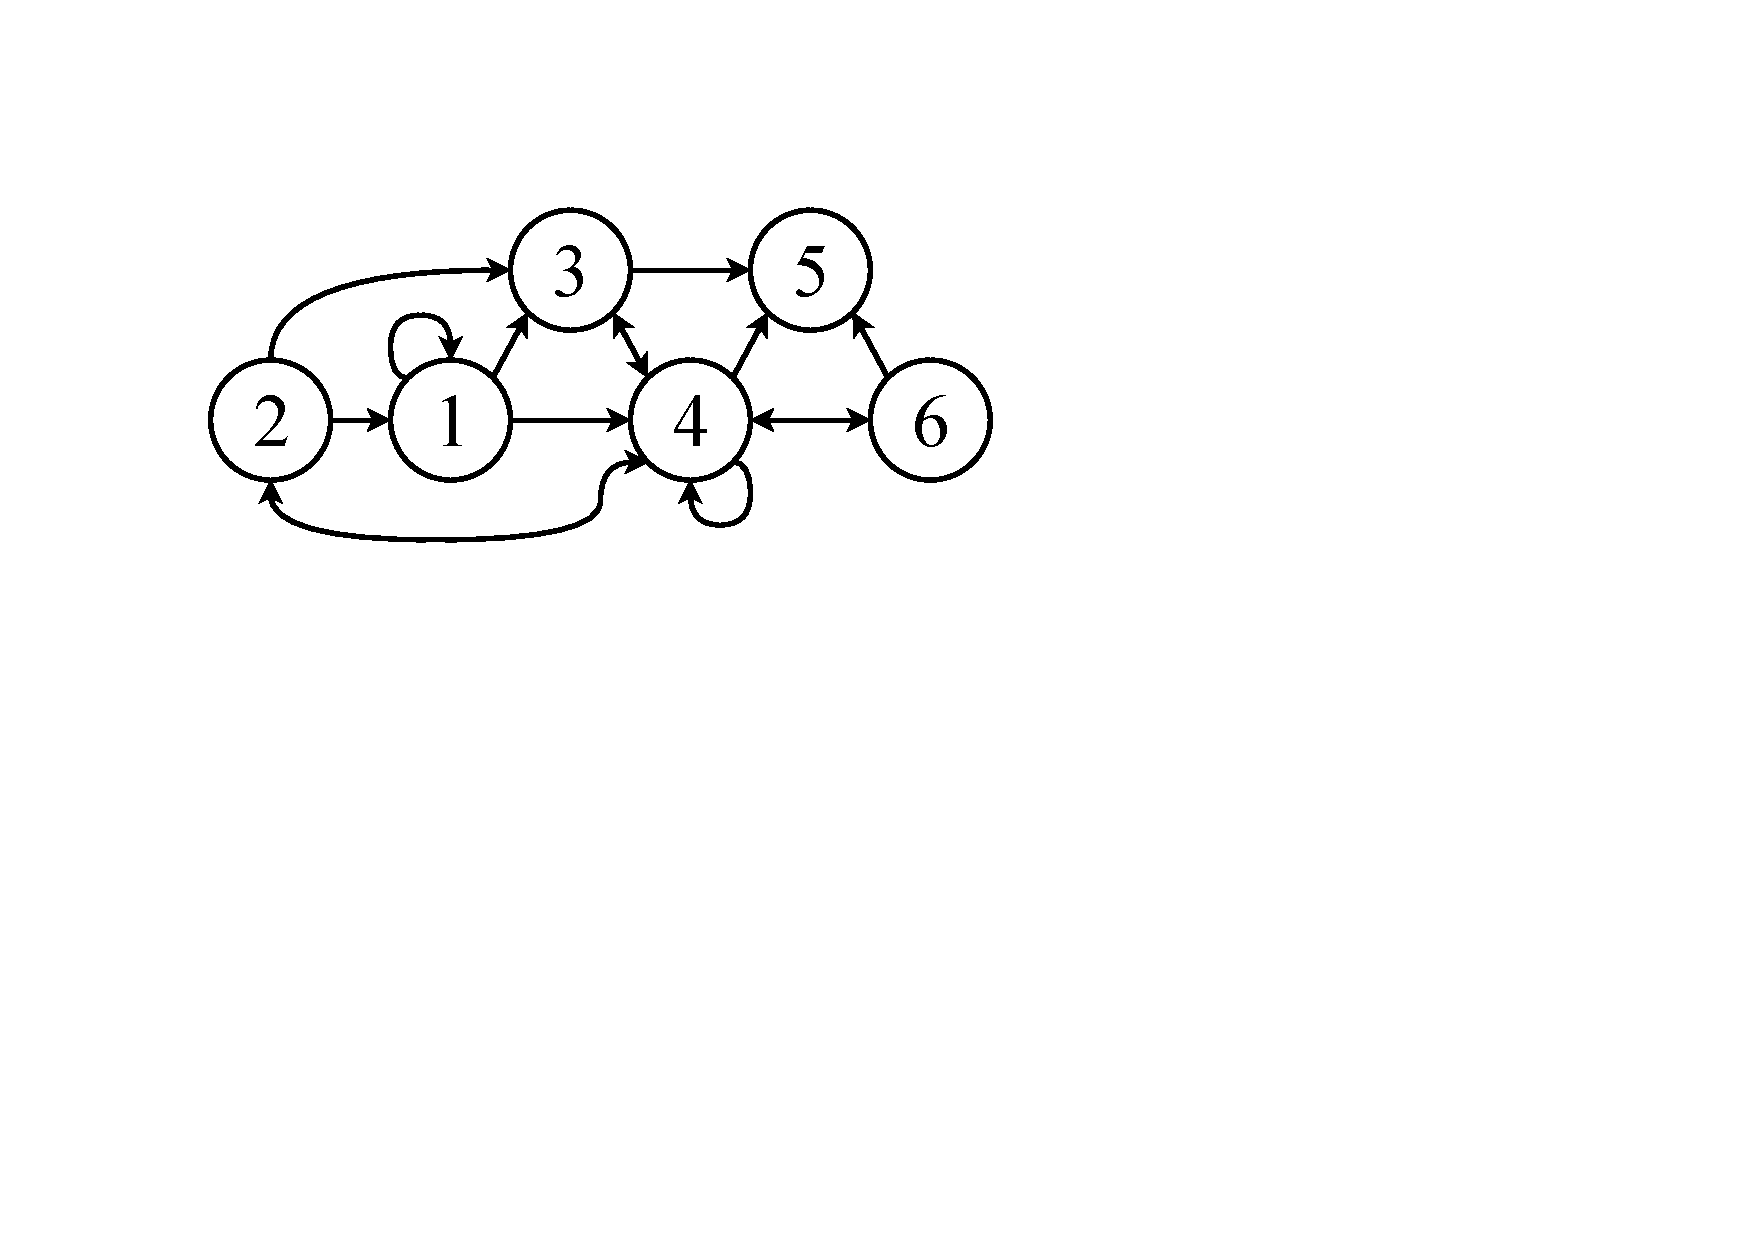
\includegraphics[scale=.2, clip,  trim=90 330 350 90]{../img/arte/graphs-repair.pdf}
    		
    			(a)
    		\end{minipage}
    		\begin{minipage}{.35\textwidth}
    			\centering
    			\footnotesize
    			\vspace{5mm}
		    	\begin{tabular}{|l|l|}
		    		\hline
		    		B1 & 111101 \\
		    		\hline
		    		B2 & 1111001\\
		    		\hline
		    	\end{tabular}
		    	\vspace{5mm}
		    	
    			(c)
    		\end{minipage}
    	\end{minipage}
    	\vspace{5mm}
    	
    	\begin{minipage}{1\textwidth}
    		\centering
    		\normalsize

		\scalebox{.65}{
		\begin{tabular}{l|l|l|l|l|l|l|l|l|l|l|l|l|l|l|l|l|l|l|l|l|l|}
			\toprule
			$T(G)$ & -1 & 1 & 3 & 4 & -2 & 1 & 3 & 4 & -3 & 4 & 5 & -4 & 3 & 4 & 5 & 6 & -5 & -6 & 4 & 5 \\
			\midrule
			$7 (4, 5)$ & -1 & 1 & 3 & 4 & -2 & 1 & 3 & 4 & -3 & 7 & -4 & 3 & 7 & 6 & -5 & -6 & 7 \\
			\cline{1-18}
			$8 (1, 3)$ & -1 & 8 & 4 & -2 & 8 & 4 & -3 & 7 & -4 & 3 & 7 & 6 & -5 & -6 & 7 \\
			\cline{1-16}
			$9 (8, 4)$ & -1 & 9 & -2 & 9 & -3 & 7 & -4 & 3 & 7 & 6 & -5 & -6 & 7 \\
			\cline{1-14}
			No $<0$ & 9 & 9 & 7 & 3 & 7 & 6 & 7 \\
			\cline{1-8}
		\end{tabular}
		}			
		\vspace{5mm}
		
		(b)
    	\end{minipage}

    \caption{Ejemplo para Re-Pair aplicado a grafos por Claude y Navarro. (a) Grafo de ejemplo. (b) Listado concatenado $T(G)$ y resultado final luego de tres reemplazos y eliminar nodos de referencia. (c) Bitmaps indicadores de nodos de referencia removidos.}
\end{figure}

\end{frame}

\begin{frame}
\frametitle{Virtual Node Mining}

\begin{figure}%[b]
    	\centering
    	\begin{minipage}{0.45\textwidth}
    		\centering
    		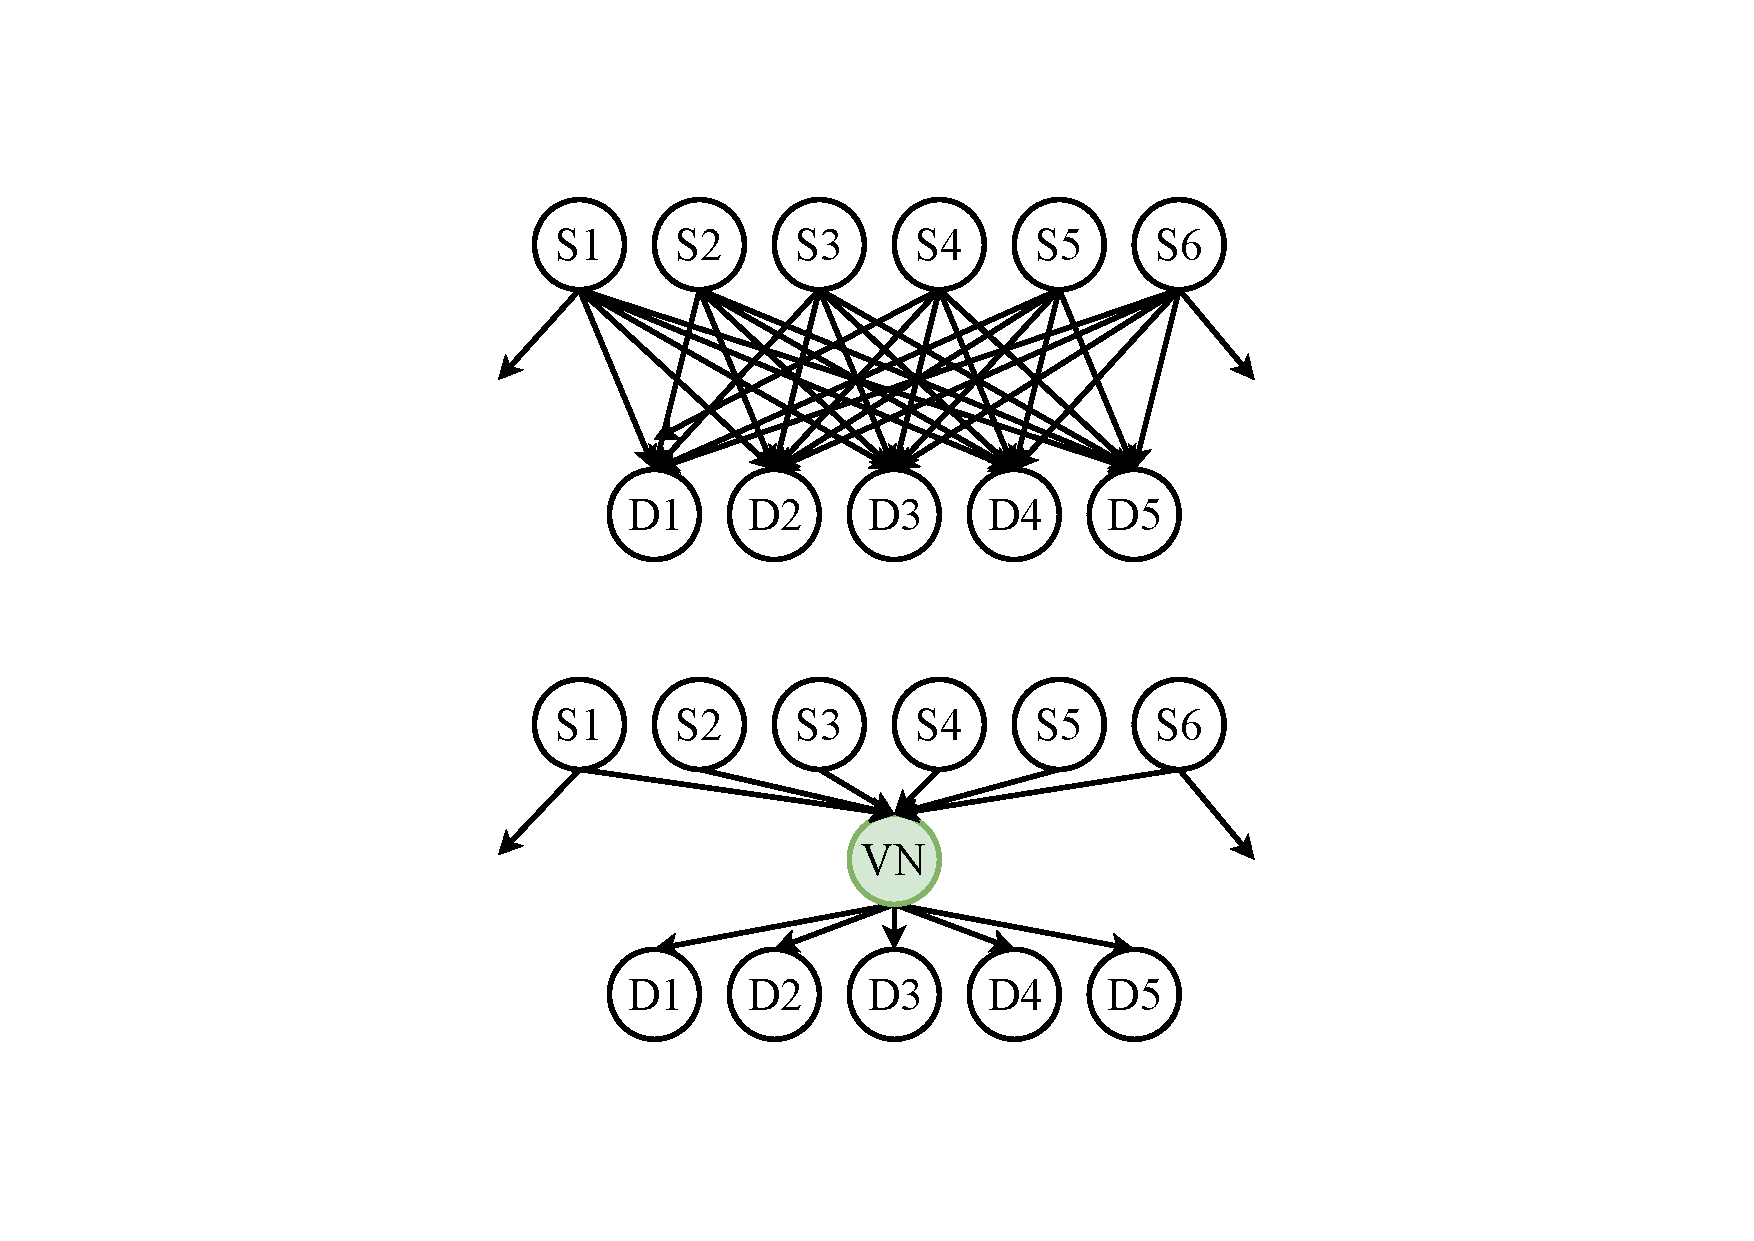
\includegraphics[scale=.3, clip,  trim=230 320 230 80]{../img/arte/graphs-virtual2.pdf}
    		
    		(a)
    	\end{minipage}
    	\begin{minipage}{0.45\textwidth}
    		\centering
    		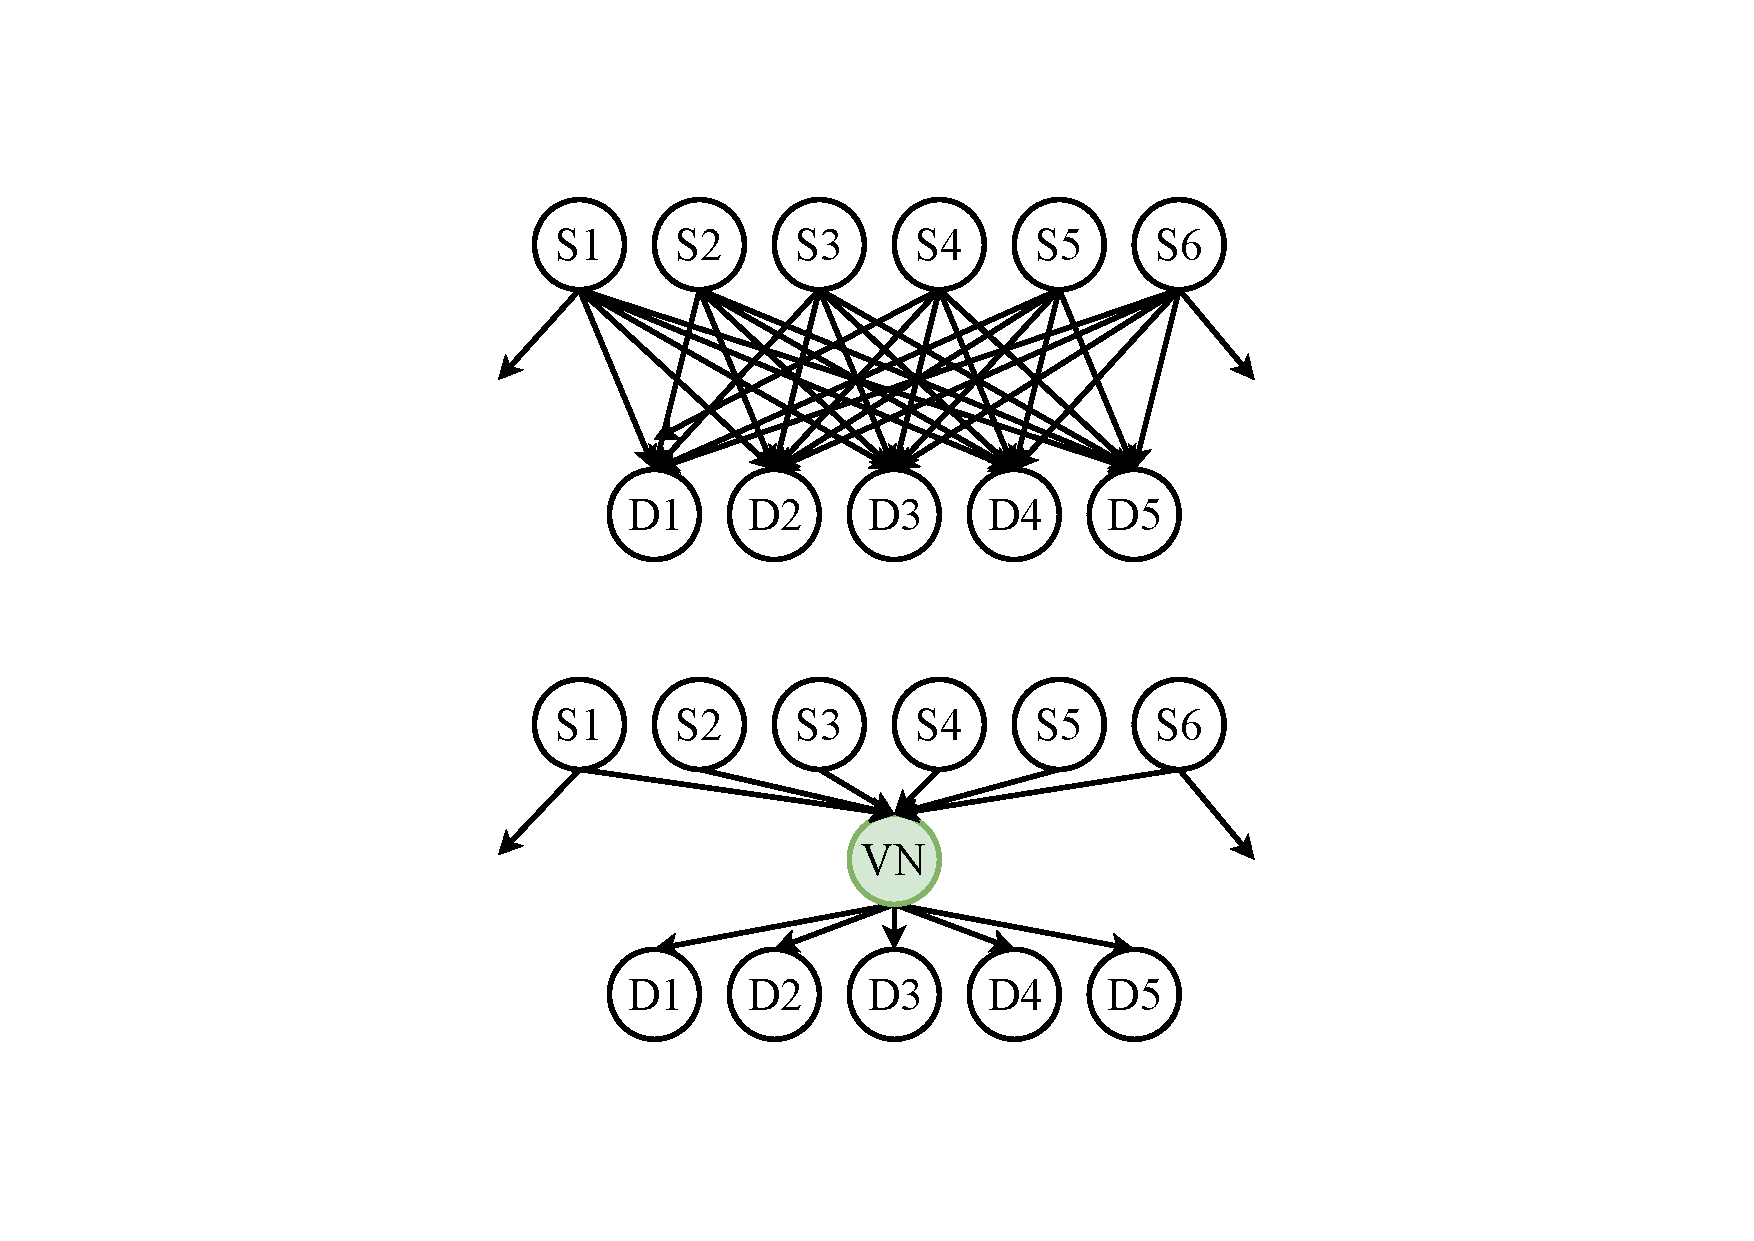
\includegraphics[scale=.3, clip,  trim=230 80 230 320]{../img/arte/graphs-virtual2.pdf}
    		
    		(b)
    	\end{minipage}

    \caption{Ejemplo de reemplazo por nodo virtual. (a) Biclique. (b) Biclique con reemplazo de aristas por nodo virtual $V$.}
\end{figure}

\end{frame}


\begin{frame}
\frametitle{k2-tree}

\begin{figure}%[b]
    	\centering
    	\begin{minipage}{0.45\textwidth}
    		\centering
    		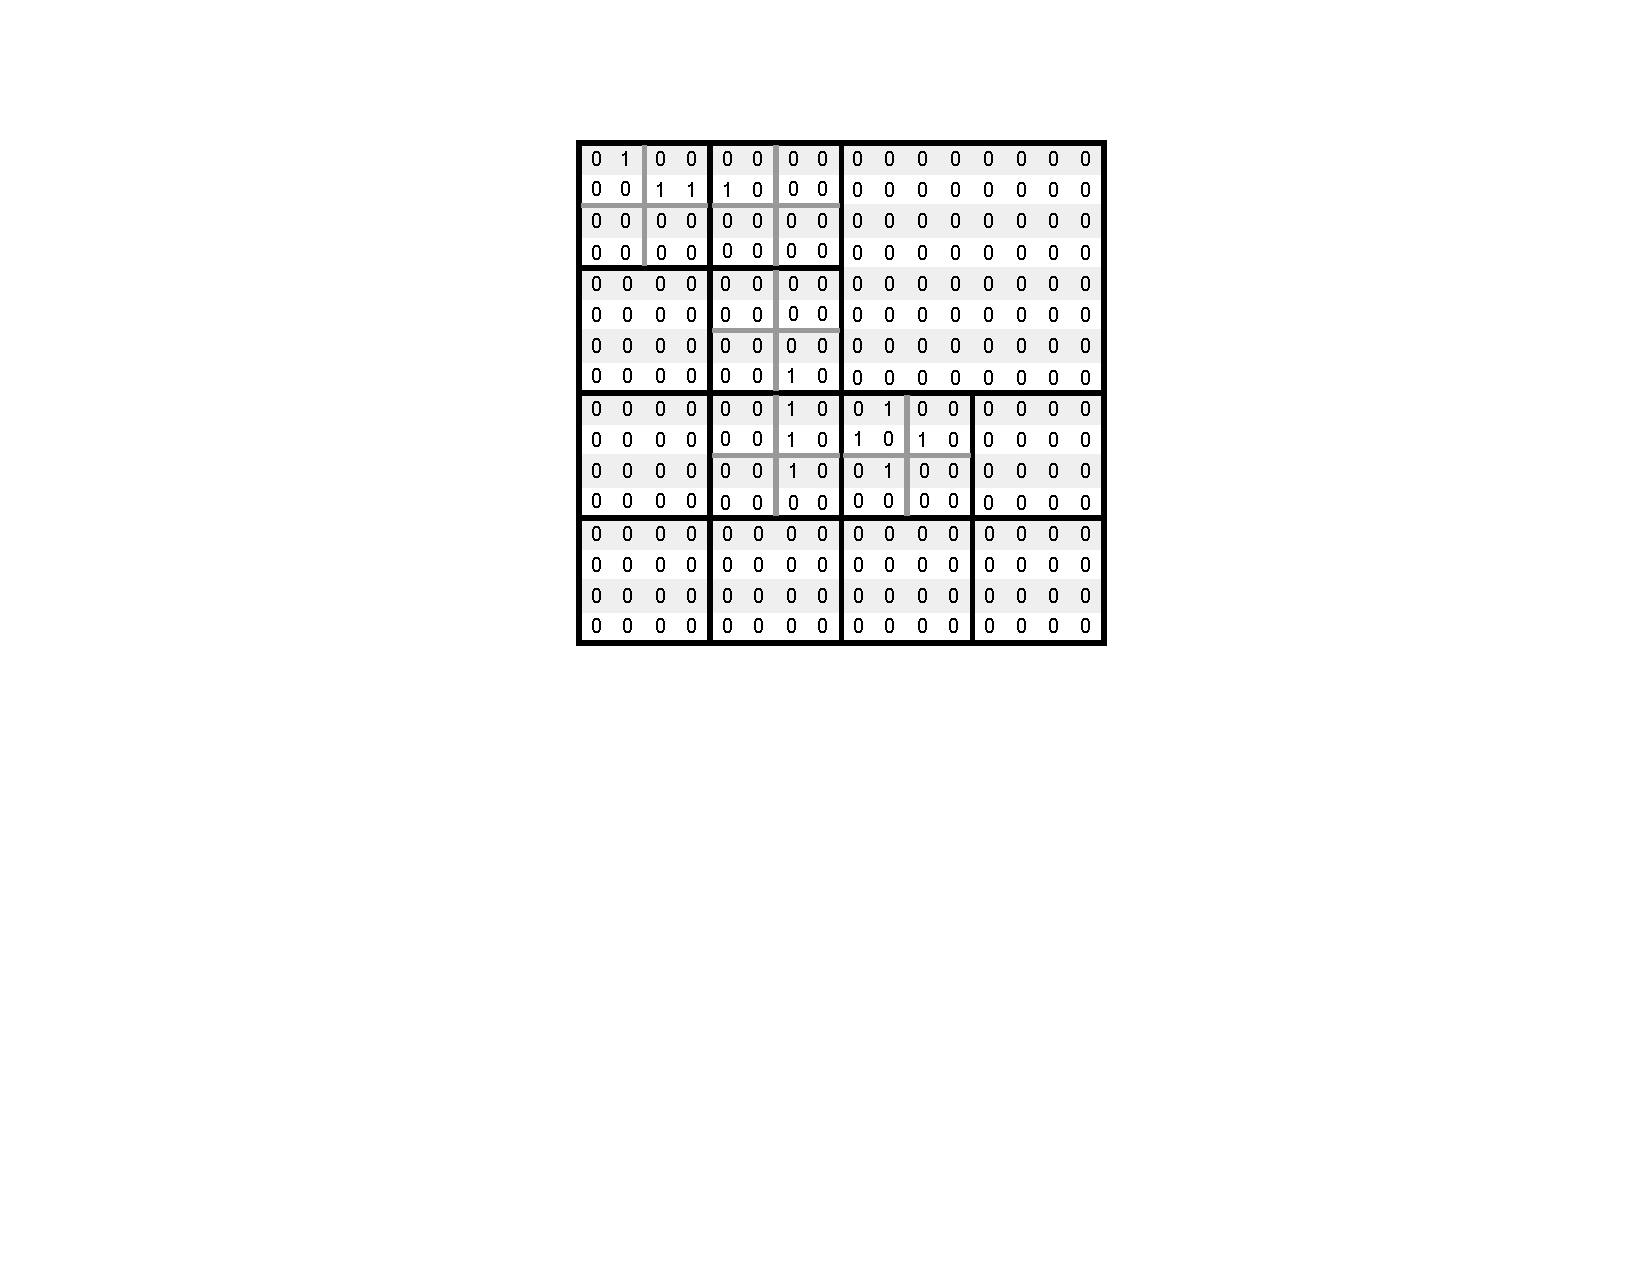
\includegraphics[scale=.5, clip,  trim=270 280 250 0]{../img/arte/k2-tree-matrix.pdf}
    		
    		(a)
    	\end{minipage}
    	\begin{minipage}{0.45\textwidth}
    		\centering
    		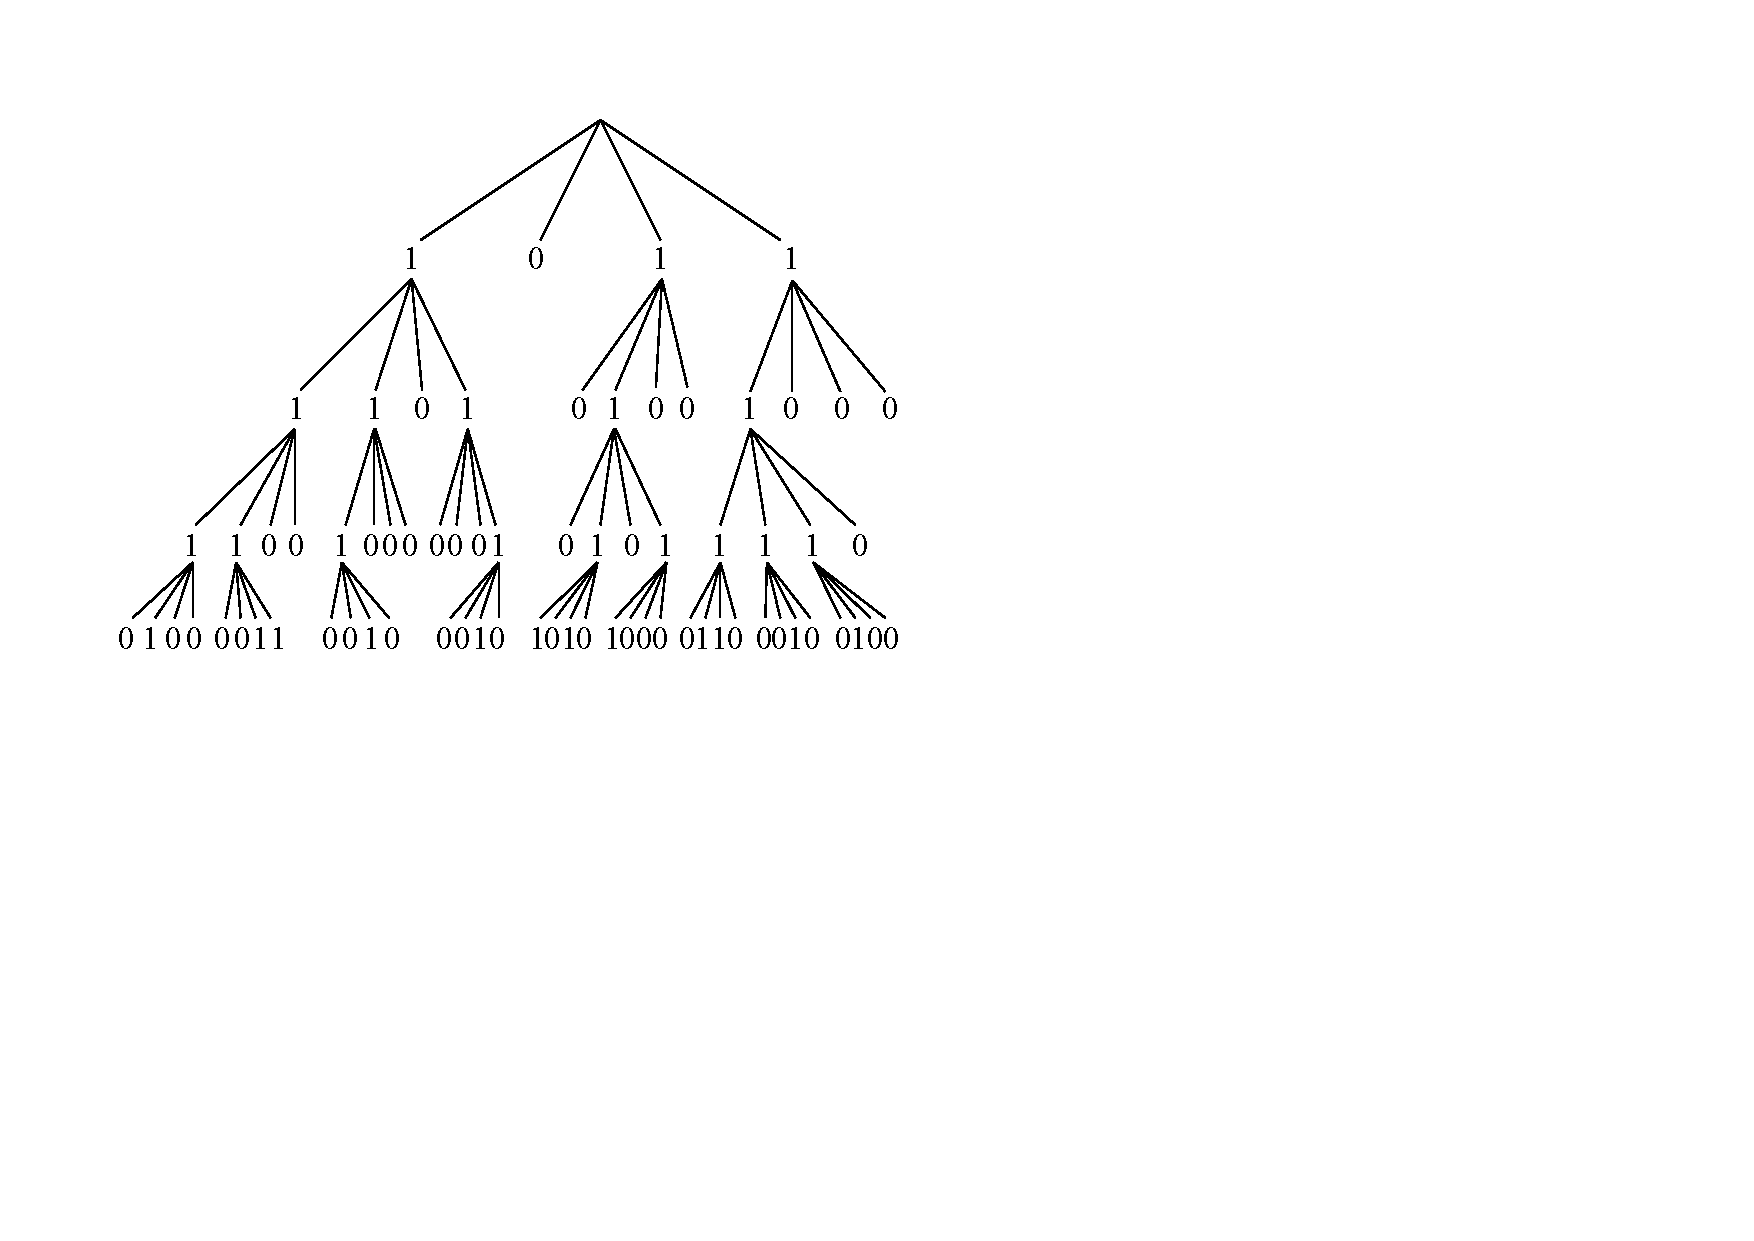
\includegraphics[scale=.4, clip, trim=50 280 410 0]{../img/arte/graphs-k2tree.pdf}
    		
    		(b)
    	\end{minipage}

    \caption{Ejemplo de k2-tree. (a) Matriz de adyacencia. (b) Diagrama de estructura.}
\end{figure}

\end{frame}



\begin{frame}
\frametitle{Wavelet tree}

\begin{figure}%[b]
    	\centering
    	\begin{minipage}{0.4\textwidth}
    		\centering
    		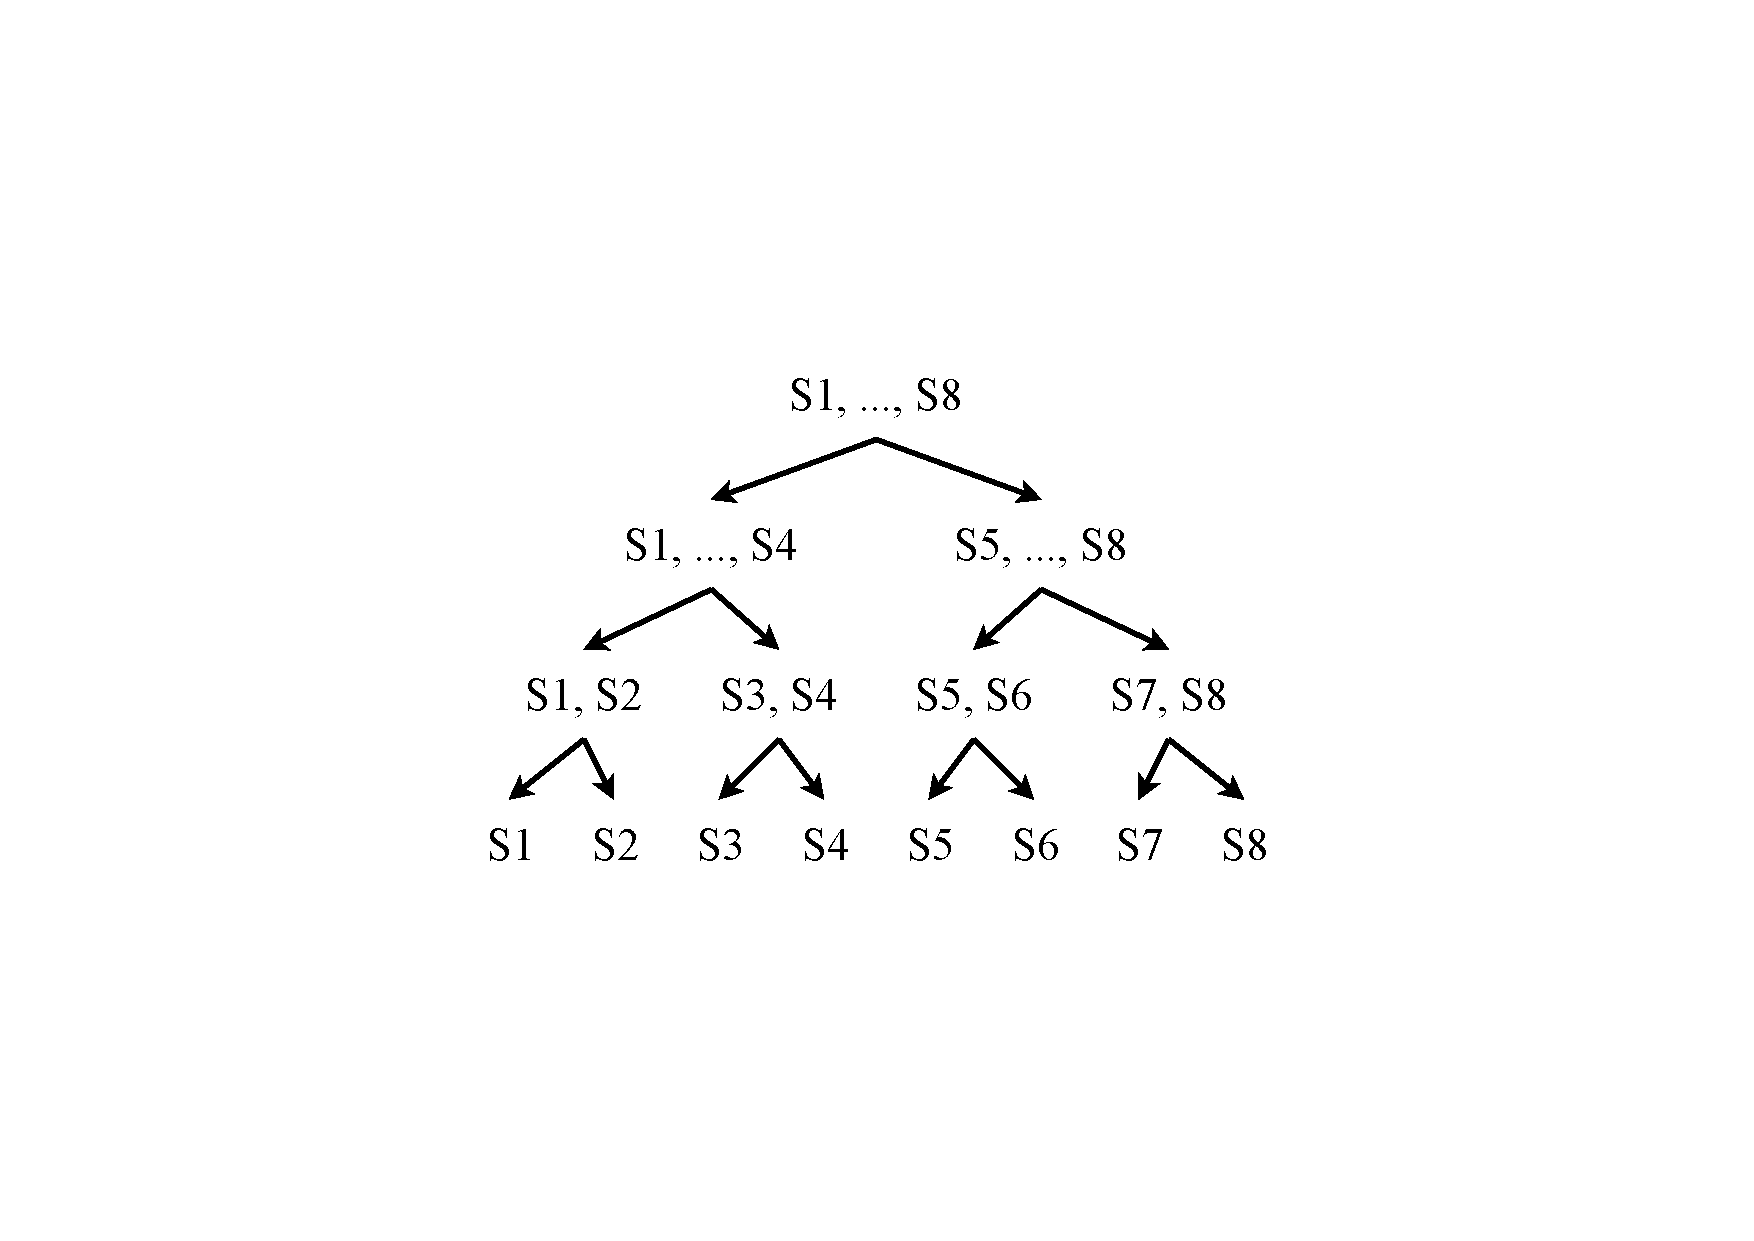
\includegraphics[scale=.3, clip,  trim=230 182 230 180]{../img/arte/graphs-wavelet-tree.pdf}
    		
    		(a)
    	\end{minipage}
    	\begin{minipage}{0.5\textwidth}
    		\centering
    		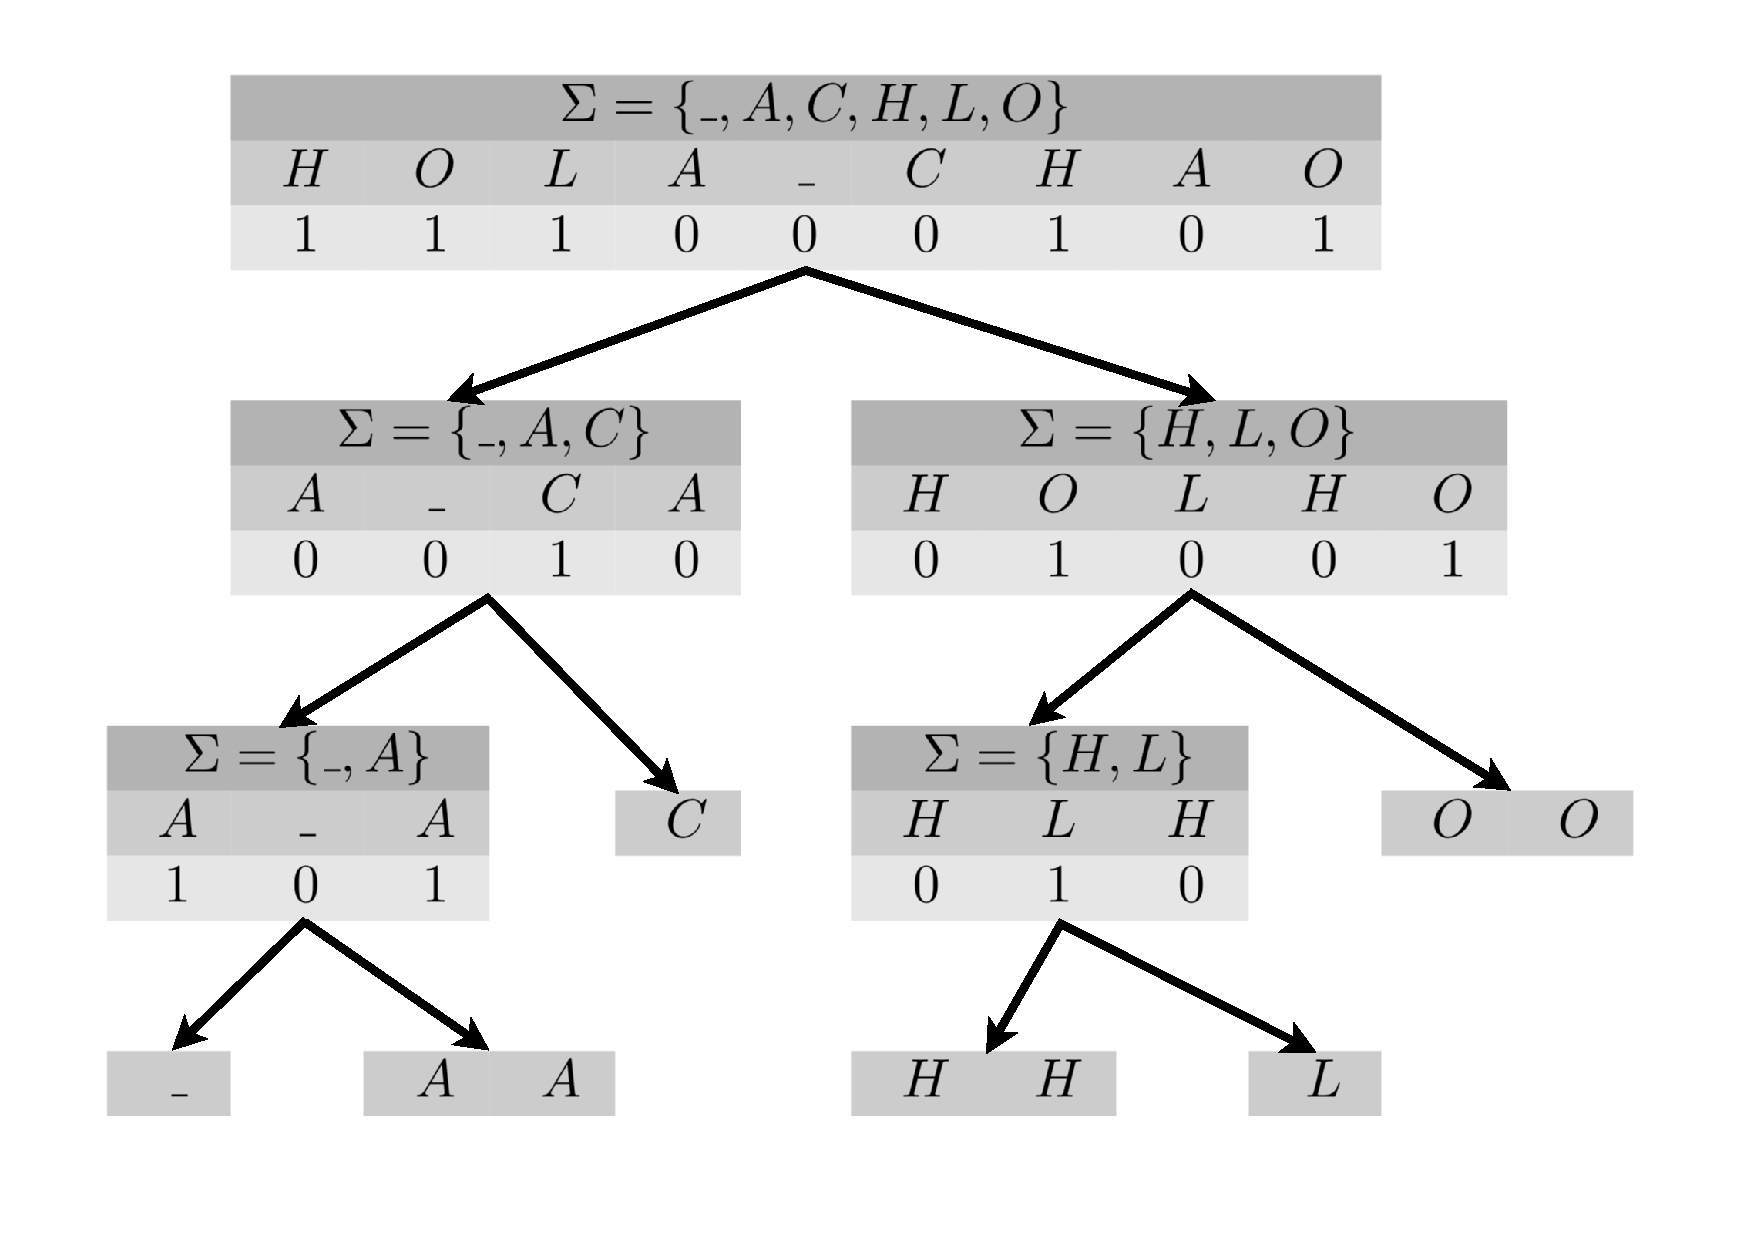
\includegraphics[scale=.2, clip, trim=0 0 0 0]{../img/arte/graphs-wavelet-tree2.pdf}

    		(b)
    	\end{minipage}

    \caption{Ejemplos de wavelet-tree. (a) Ejemplo básico de subdivisión de secuencia ordenada. (b) Ejemplo práctico con alfabetos y bitmaps por nodo.}
\end{figure}

\end{frame}


\begin{frame}
\frametitle{Wavelet matrix}

\begin{figure}%[b]
    	\centering
    	\begin{minipage}{0.3\textwidth}
    		\centering
    		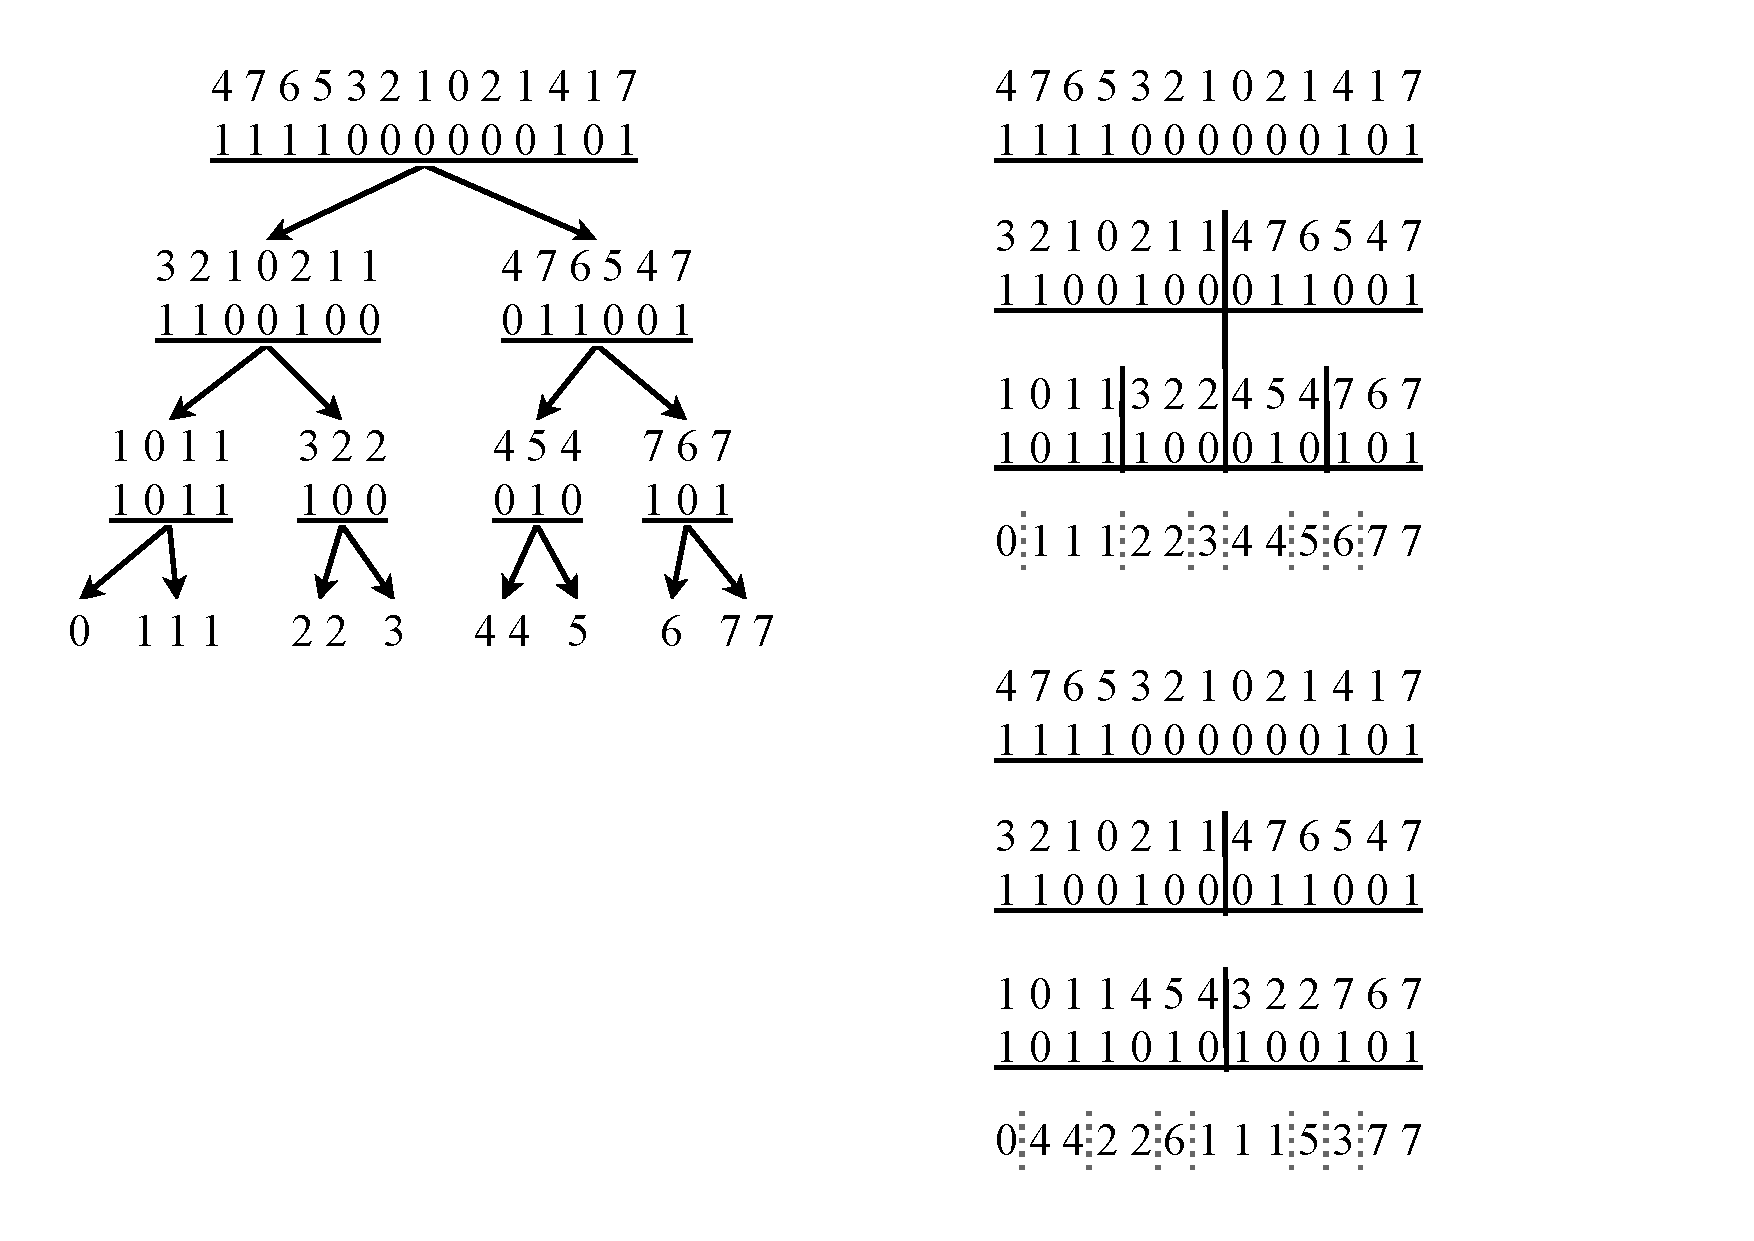
\includegraphics[scale=.3, clip,  trim=30 280 440 30]{../img/arte/graphs-wavelet-matrix.pdf}
    		
    		(a)
    	\end{minipage}
    	\begin{minipage}{0.3\textwidth}
    		\centering
    		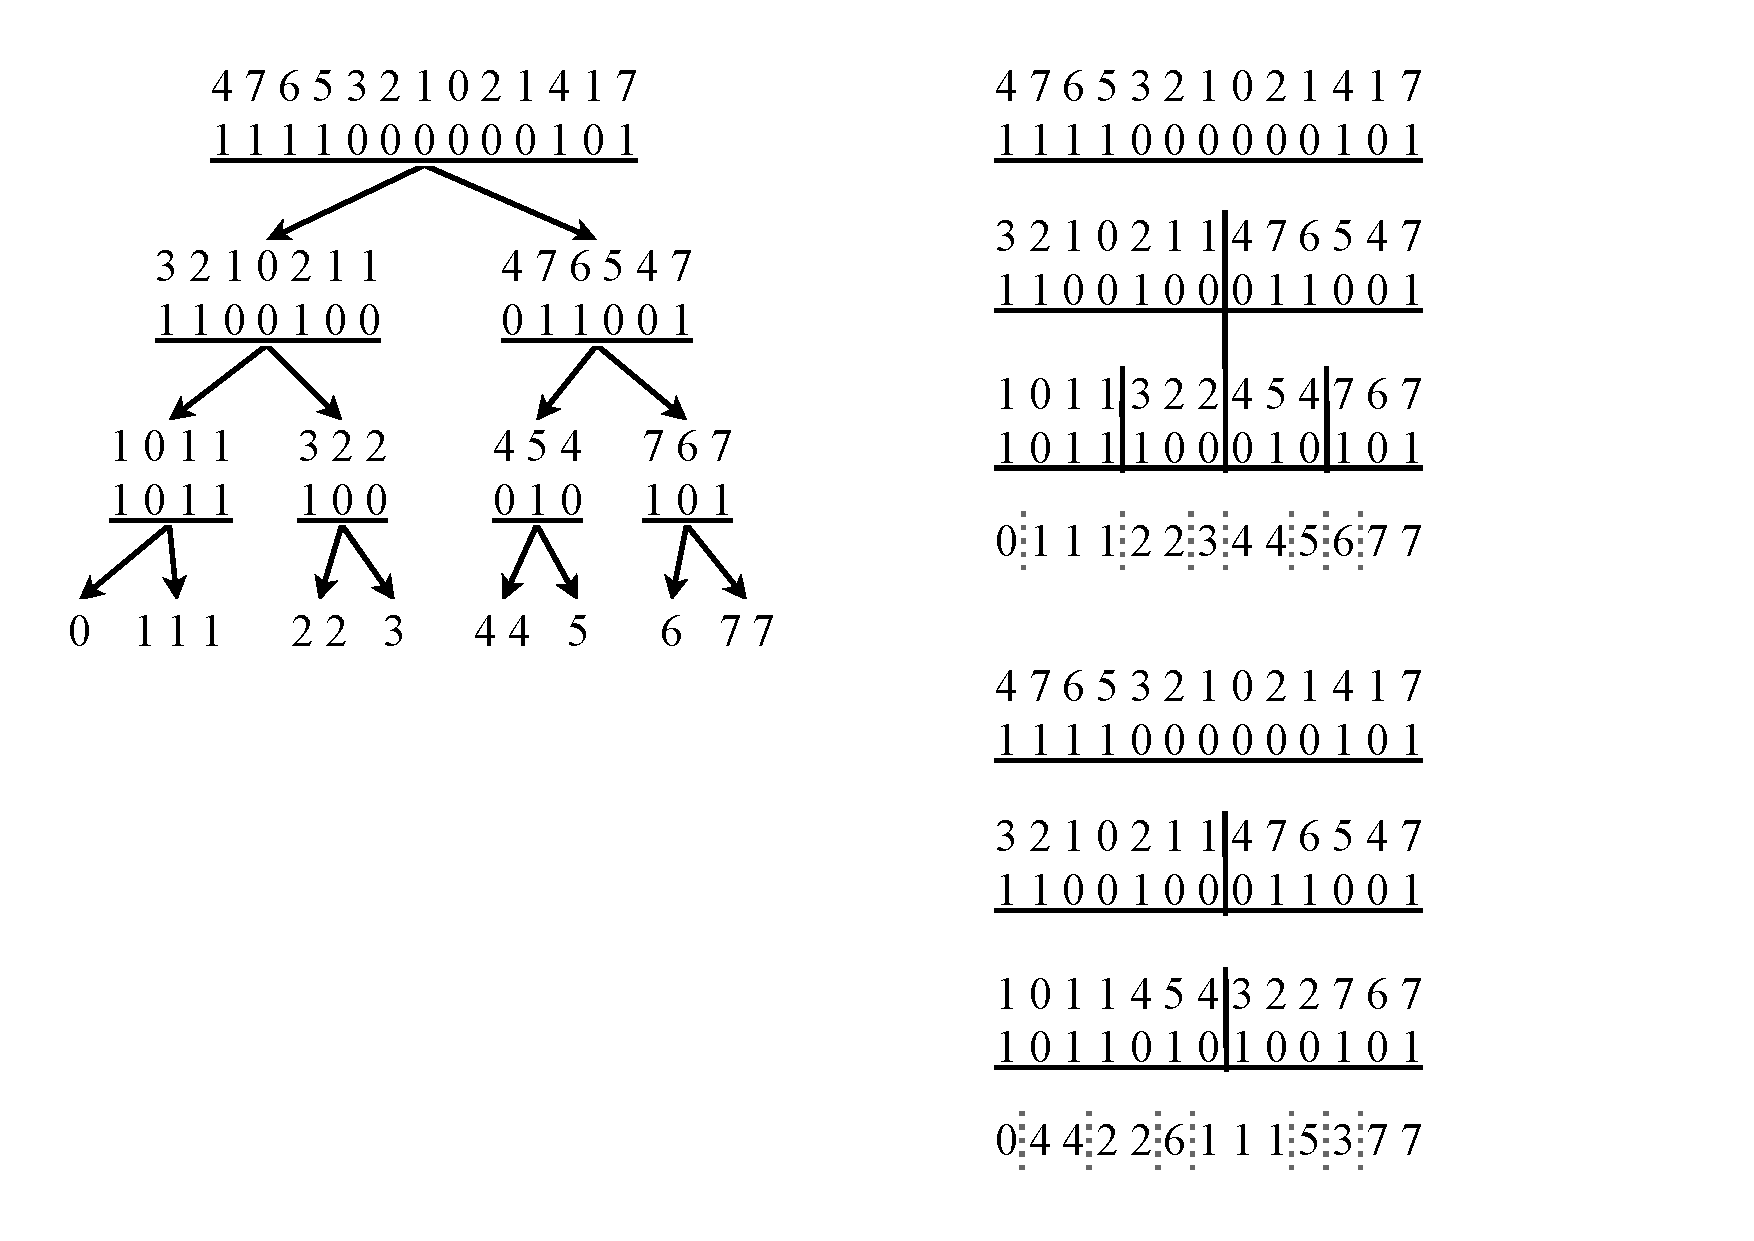
\includegraphics[scale=.3, clip, trim=470 320 170 30]{../img/arte/graphs-wavelet-matrix.pdf}

    		(b)
    	\end{minipage}
    	\begin{minipage}{0.3\textwidth}
    		\centering
    		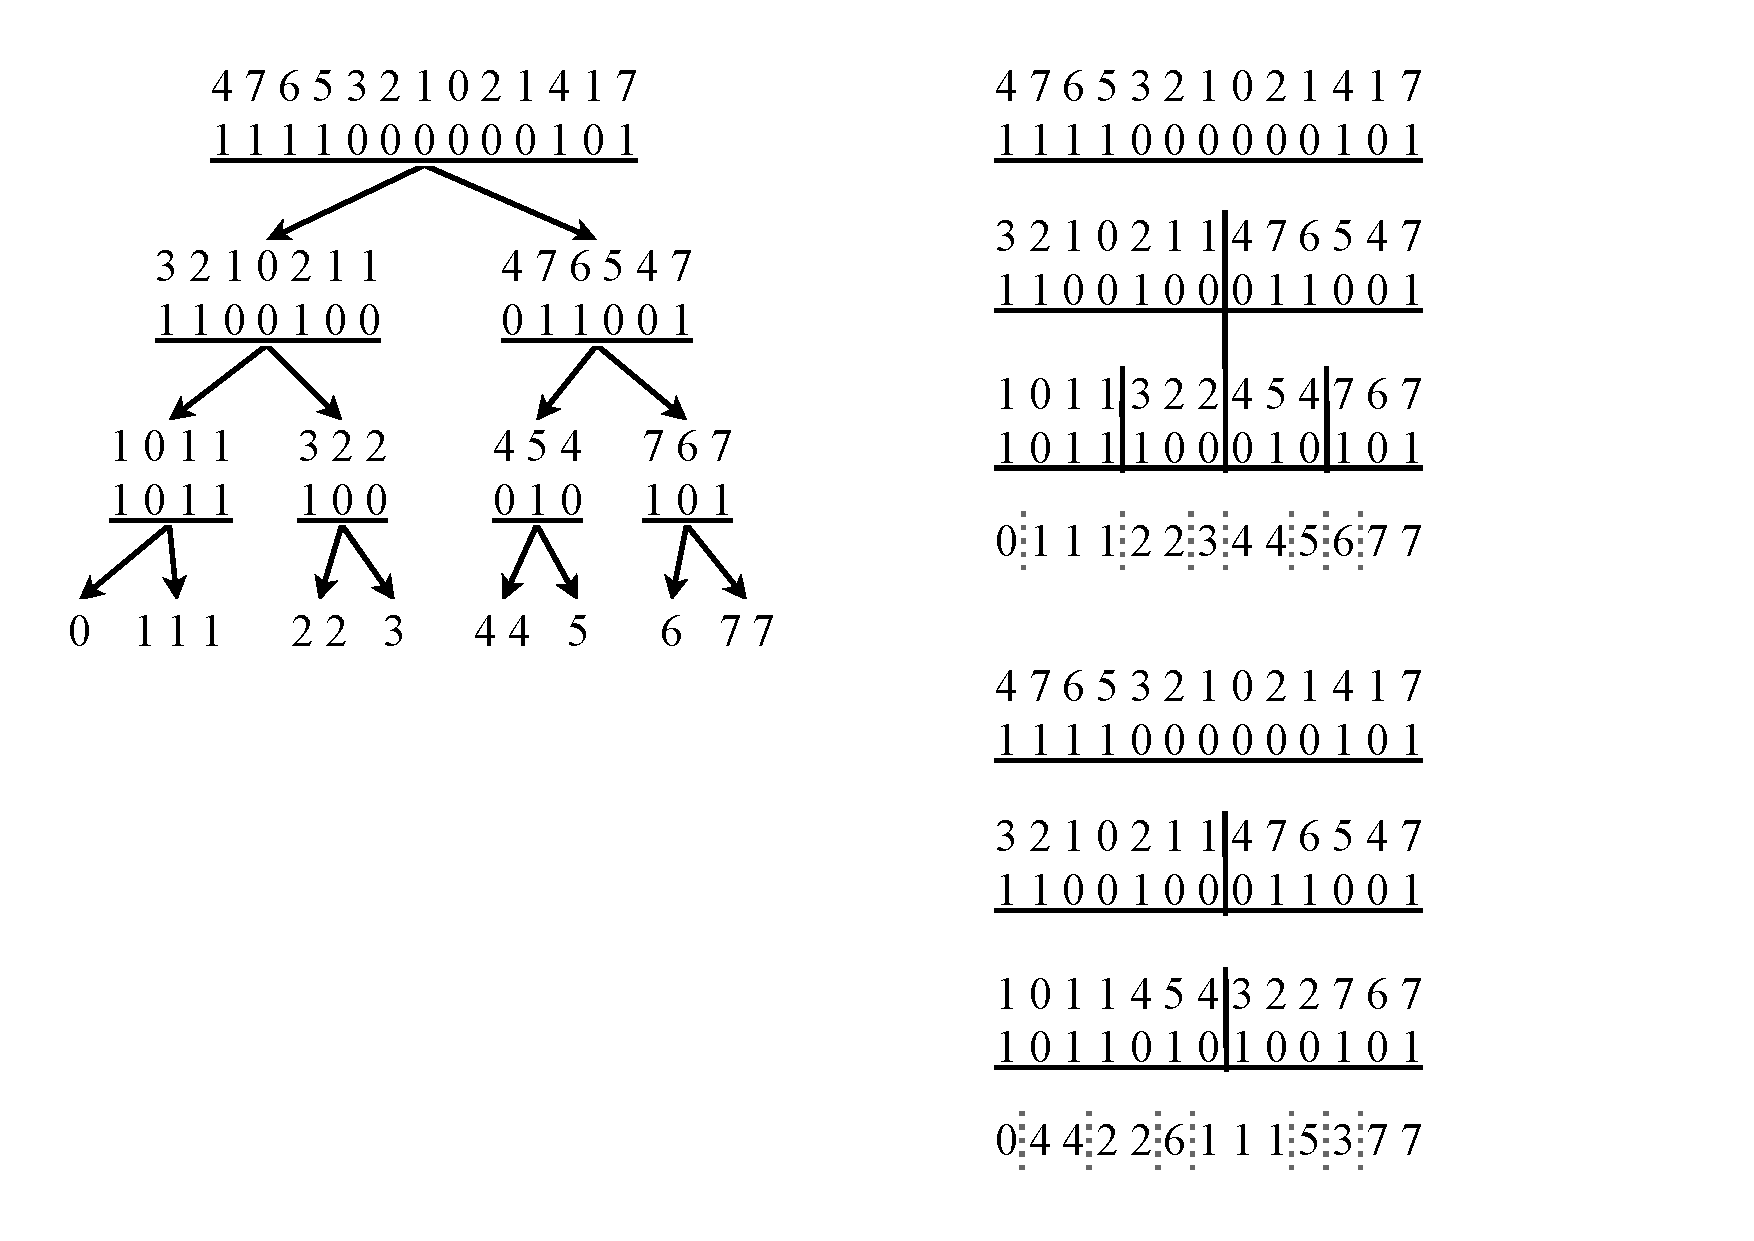
\includegraphics[scale=.3, clip, trim=470 33 170 317]{../img/arte/graphs-wavelet-matrix.pdf}

    		(c)
    	\end{minipage}

    \caption{Ejemplos para wavelet-matrix. (a) Un wavelet tree. (b) El mismo wavelet tree sin punteros. (c) La wavelet matrix correpondiente.}
\end{figure}

\end{frame}